\documentclass[../../main.tex]{subfiles}
\begin{document}

$xy$ 平面において放物線 $y=x^2$ の，$0<x<1$ に対応する部分を $L$ とする．
(すなわち $L= \{ (x,x^2) \mid 0<x<1 \}$ である．)
点 $P(x,x^2)$ における $L$ の接線が直線 $y=0$，直線 $x=1$ と交わる点をそれぞれ $A$，$B$ とする．
また座標が $(0,0)$，$(1,0)$，$(1,1)$ である三点を，
それぞれ $O$，$C$，$D$ とする．

以下つねに $0<x<1$ という範囲で考えるものとする．

\begin{figure}[H]
  \centering
  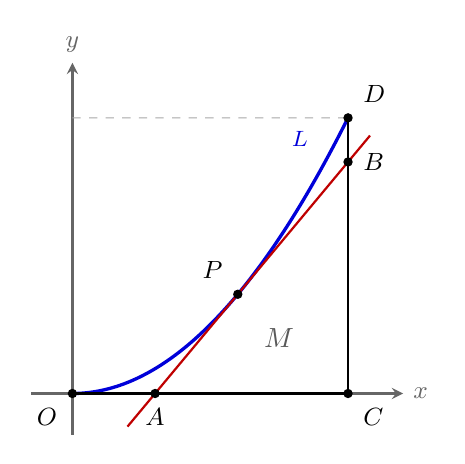
\begin{tikzpicture}[scale=3.5, >=stealth, every node/.style={font=\small}]
    \coordinate (O) at (0,0);
    \coordinate (C) at (1,0);
    \coordinate (D) at (1,1);

    % 座標軸
    \draw[->, thick, gray!80!black] (-0.15, 0) -- (1.2, 0) node[right] {$x$};
    \draw[->, thick, gray!80!black] (0, -0.15) -- (0, 1.2) node[above] {$y$};

    % 放物線 L: y = x^2 (0 < x < 1)
    \draw[very thick, blue!85!black, domain=0:1, samples=60] plot (\x, {\x*\x});
    \node[blue!85!black, above left=1pt, font=\footnotesize] at (0.9, 0.85) {$L$};

    % 線分 OC, CD
    \draw[thick] (O) -- (C) -- (D);
    \draw[dashed, gray!70] (0, 1) -- (D);

    % 領域 M
    \node[gray!70!black, font=\bfseries] at (0.75, 0.2) {$M$};

    % 点 P (x=0.6, y=0.36) における接線
    \def\xP{0.6}
    \pgfmathsetmacro{\yP}{\xP * \xP}
    \pgfmathsetmacro{\xA}{0.5 * \xP}
    \pgfmathsetmacro{\yB}{2.0*\xP - \yP}
    \coordinate (P) at (\xP, \yP);
    \coordinate (A) at (\xA, 0);
    \coordinate (B) at (1, \yB);

    \draw[thick, red!75!black] (\xA - 0.1, {-0.1*2*\xP}) -- (1.08, {\yB + 0.08*2*\xP});

    % 点のプロットとラベル
    \node[circle, fill, inner sep=1.2pt] at (O) {}; \node[below left=2pt] at (O) {$O$};
    \node[circle, fill, inner sep=1.2pt] at (C) {}; \node[below right=2pt] at (C) {$C$};
    \node[circle, fill, inner sep=1.2pt] at (D) {}; \node[above right=2pt] at (D) {$D$};
    \node[circle, fill, inner sep=1.2pt] at (P) {}; \node[above left=2pt] at (P) {$P$};
    \node[circle, fill, inner sep=1.2pt] at (A) {}; \node[below=2pt] at (A) {$A$};
    \node[circle, fill, inner sep=1.2pt] at (B) {}; \node[right=2pt] at (B) {$B$};
  \end{tikzpicture}
  \caption{問題の図}
  \label{fig:problem}
\end{figure}

\begin{enumerate}
  \item $\triangle PAC$，$\triangle PCB$ の面積をそれぞれ $g(x)$，$h(x)$ とするとき，
    $g(x) \leqq h(x)$ となる $x$ の範囲を求めよ．

  \item 線分 $OC$ および線分 $CD$ と放物線の一部 $L$ で囲まれた範囲を $M$ とする．
    ただし $M$ はその周である線分 $OC$，$CD$ および $L$ を含むものとする．
    いま $L$ 上の点 $P(x,x^2)$ を頂点とし，$M$ に含まれるような三角形のうちで，
    最大の面積を持つものの面積を $f(x)$ とする．
    関数 $f(x)$ を求め，そのグラフを描け．
    また $f(x)$ の極値を求めよ．
    ただし $I=\{ x \mid 0<x<1 \}$ の点 $a$ で，関数 $f$ が極小値(または極大値)をとるとは，
    $a$ に近い $I$ のすべての点 $x$ に対して $f(a) \leqq f(x)$ (または $f(a) \geqq f(x)$) となることをいう．
    極大値と極小値をあわせて極値という．
\end{enumerate}

\end{document}
